\chapter{Gestione del cluster con un algoritmo di controllo dinamico}
In questo capitolo si analizza come la gestione del cluster di nove incroci interconnessi presentato in precedenza, con un algoritmo di controllo dinamico, riesca a ridurre le congestioni, creando un flusso di veicoli più omogeneo, con tempi di attesa minori e generalmente uniformi, e con un numero di macchine in coda, per ogni corsia presente (che sia essa intermedia o collegata ad un Generator) tenuto sotto controllo.

L'algoritmo utilizzato è esattamente quello presentato nel \textit{Capitolo \ref{capitolo2}} (Codice \ref{algoritmodin}). Questo è stato applicato singolarmente ad ogni incrocio, che lavora in maniera autonoma. Dunque ogni giunzione non ha alcuna coscienza di essere inserita in una simulazione più ampia, e ciò migliora l'espandibilità del modello, essendo appunto ogni incrocio indipendente da tutti gli altri.

Riassumendo, non si è voluto che le giunzioni scambiassero dati fra loro per verificare se queste riuscissero autonomamente a sincronizzarsi e regolarsi al meglio, e si è osservato che in effetti la tendenza è proprio questa: anche senza sapere nulla del contesto circostante, ogni incrocio, applicando in autonomia l'algoritmo già più volte spiegato, riesce ad apportare un contributo all'intero cluster in termini di miglioramento della gestione del flusso automobilistico.
\newpage

\section{Il modello di confronto}
Anche in questo caso, per effettuare un confronto fra una gestione "canonica" ed una gestione ottimizzata si è scelto di creare un modello apposito, in cui ogni Generator viene collegato ad un Entity Replicator, che crea due repliche dell'entità in ingresso (l'automobile) inviandone una al cluster gestito staticamente e l'altra a quello i cui incroci implementano l'algoritmo. 

In questo modo i due cluster hanno esattamente gli stessi input, pertanto si può effettuare un confronto puntuale e preciso su chi stia gestendo meglio il flusso e quali parametri stia ottimizzando.
\newline

Nella realizzazione del modello non ci si è discostati da quanto detto nel \textit{Capitolo \ref{capitolo2}} (\textit{Paragrafo 2.4}), semplicemente si è esteso il concetto presentato in precedenza all'intero cluster ed a tutti gli Entity Generator presenti. Per questo motivo non si entrerà nello specifico nella spiegazione del suddetto modello, il cui schema è riportato alla pagina seguente.
\newpage

\section{I risultati ottenuti}
Nel precedente capitolo è stata analizzata una simulazione considerando esclusivamente i risultati ottenuti con una gestione statica. Ora, a partire dagli stessi dati, viene presentata anche la gestione dinamica ed ottimizzata dello stesso flusso di auto in una tabella di confronto riassuntiva. Si può da subito notare come in tutte le corsie vi sia un miglioramento, in alcuni casi molto marcato, soprattutto per quelle collegate ai Generator, in altri lieve ma comunque presente. Dai grafici successivi è ancora più facile comprendere quanto si sta affermando, e come non vi sia alcun motivo per non implementare un meccanismo di gestione come quello presentato in questo lavoro di tesi per gestire al meglio gli incroci cittadini.
\begin{table}[H]
\centering
\begin{tabular}{|C{2.2cm}|C{2.2cm}|C{2.9cm}|C{2.9cm}|C{2.9cm}|}
\hline
\textbf{Corsia} &
\textbf{Tipologia} &
\textbf{Max numero auto in coda} &
\textbf{Tempo di attesa medio} &
\textbf{Numero di auto totale} \\\hline
\multirow{3}{2.2cm}{\centering \footnotesize{[1 - 1] Ovest - Dritto-Destra}} &
\footnotesize{Generator (Statico)} &
12 &
42.81 &
2550 \\\cline{2-5}
&
\footnotesize{Generator (Dinamico)} &
8 &
16.42 &
2551 \\\hline
\multirow{3}{2.2cm}{\centering \footnotesize{[1 - 1] Ovest - Sinistra}} &
\footnotesize{Generator (Statico)} &
15 &
49.27 &
2647 \\\cline{2-5}
&
\footnotesize{Generator (Dinamico)} &
10 &
18.94 &
2650 \\\hline
\multirow{3}{2.2cm}{\centering \footnotesize{[1 - 1] Nord - Dritto-Destra}} &
\footnotesize{Generator (Statico)} &
11 &
38.01 &
2301 \\\cline{2-5}
&
\footnotesize{Generator (Dinamico)} &
9 &
20.77 &
2301 \\\hline
\multirow{3}{2.2cm}{\centering \footnotesize{[1 - 1] Nord - Sinistra}} &
\footnotesize{Generator (Statico)} &
12 &
37.63 &
2402 \\\cline{2-5}
&
\footnotesize{Generator (Dinamico)} &
7 &
18.96 &
2402 \\\hline
\multirow{3}{2.2cm}{\centering \footnotesize{[1 - 1] Est - Dritto-Destra}} &
\footnotesize{Terminator (Statico)} &
9 &
21.96 &
2346 \\\cline{2-5}
&
\footnotesize{Terminator (Dinamico)} &
8 &
19.76 &
2346 \\\hline
\multirow{3}{2.2cm}{\centering \footnotesize{[1 - 1] Est - Sinistra}} &
\footnotesize{Intermedio (Statico)} &
10 &
21.95 &
2402 \\\cline{2-5}
&
\footnotesize{Intermedio (Dinamico)} &
10 &
21.39 &
2401 \\\hline
\multirow{3}{2.2cm}{\centering \footnotesize{[1 - 1] Sud - Dritto-Destra}} &
\footnotesize{Terminator (Statico)} &
9 &
23.79 &
2427 \\\cline{2-5}
&
\footnotesize{Terminator (Dinamico)} &
6 &
26.42 &
2430 \\\hline
\multirow{3}{2.2cm}{\centering \footnotesize{[1 - 1] Sud - Sinistra}} &
\footnotesize{Terminator (Statico)} &
10 &
27.48 &
2416 \\\cline{2-5}
&
\footnotesize{Terminator (Dinamico)} &
10 &
25.44 &
2417 \\\hline
\multirow{3}{2.2cm}{\centering \footnotesize{[1 - 2] Ovest - Dritto-Destra}} &
\footnotesize{Intermedio (Statico)} &
10 &
52.48 &
2510 \\\cline{2-5}
&
\footnotesize{Intermedio (Dinamico)} &
9 &
16.77 &
2513 \\\hline
\end{tabular}
\caption{Confronto fra gestione statica e dinamica di un cluster di nove incroci - pt.1}
\label{table:keytable}
\end{table}
\newpage
\begin{table}[H]
\centering
\begin{tabular}{|C{2.2cm}|C{2.2cm}|C{2.9cm}|C{2.9cm}|C{2.9cm}|}
\hline
\textbf{Corsia} &
\textbf{Tipologia} &
\textbf{Max numero auto in coda} &
\textbf{Tempo di attesa medio} &
\textbf{Numero di auto totale} \\\hline
\multirow{3}{2.2cm}{\centering \footnotesize{[1 - 2] Ovest - Sinistra}} &
\footnotesize{Terminator (Statico)} &
9 &
45.73 &
2264 \\\cline{2-5}
&
\footnotesize{Terminator (Dinamico)} &
7 &
17.87 &
2265 \\\hline
\multirow{3}{2.2cm}{\centering \footnotesize{[1 - 2] Nord - Dritto-Destra}} &
\footnotesize{Generator (Statico)} &
11 &
38.84 &
2342 \\\cline{2-5}
&
\footnotesize{Generator (Dinamico)} &
7 &
20.26 &
2345 \\\hline
\multirow{3}{2.2cm}{\centering \footnotesize{[1 - 2] Nord - Sinistra}} &
\footnotesize{Generator (Statico)} &
9 &
35.20 &
2219 \\\cline{2-5}
&
\footnotesize{Generator (Dinamico)} &
9 &
19.06 &
2223 \\\hline
\multirow{3}{2.2cm}{\centering \footnotesize{[1 - 2] Est - Dritto-Destra}} &
\footnotesize{Intermedio (Statico)} &
10 &
23.95 &
2306 \\\cline{2-5}
&
\footnotesize{Intermedio (Dinamico)} &
9 &
19.13 &
2306 \\\hline
\multirow{3}{2.2cm}{\centering \footnotesize{[1 - 2] Est - Sinistra}} &
\footnotesize{Intermedio (Statico)} &
7 &
22.83 &
2329 \\\cline{2-5}
&
\footnotesize{Intermedio (Dinamico)} &
8 &
21.67 &
2329 \\\hline
\multirow{3}{2.2cm}{\centering \footnotesize{[1 - 2] Sud - Dritto-Destra}} &
\footnotesize{Terminator (Statico)} &
10 &
52.39 &
2488 \\\cline{2-5}
&
\footnotesize{Terminator (Dinamico)} &
7 &
25.08 &
2488 \\\hline
\multirow{3}{2.2cm}{\centering \footnotesize{[1 - 2] Sud - Sinistra}} &
\footnotesize{Intermedio (Statico)} &
10 &
46.14 &
2407 \\\cline{2-5}
&
\footnotesize{Intermedio (Dinamico)} &
7 &
23.67 &
2407 \\\hline
\multirow{3}{2.2cm}{\centering \footnotesize{[1 - 3] Ovest - Dritto-Destra}} &
\footnotesize{Terminator (Statico)} &
10 &
46.32 &
2330 \\\cline{2-5}
&
\footnotesize{Terminator (Dinamico)} &
6 &
15.55 &
2332 \\\hline
\multirow{3}{2.2cm}{\centering \footnotesize{[1 - 3] Ovest - Sinistra}} &
\footnotesize{Terminator (Statico)} &
10 &
47.46 &
2311 \\\cline{2-5}
&
\footnotesize{Terminator (Dinamico)} &
7 &
17.63 &
2312 \\\hline
\end{tabular}
\caption{Confronto fra gestione statica e dinamica di un cluster di nove incroci - pt.2}
\label{table:keytable}
\end{table}
\newpage
\begin{table}[H]
\centering
\begin{tabular}{|C{2.2cm}|C{2.2cm}|C{2.9cm}|C{2.9cm}|C{2.9cm}|}
\hline
\textbf{Corsia} &
\textbf{Tipologia} &
\textbf{Max numero auto in coda} &
\textbf{Tempo di attesa medio} &
\textbf{Numero di auto totale} \\\hline
\multirow{3}{2.2cm}{\centering \footnotesize{[1 - 3] Nord - Dritto-Destra}} &
\footnotesize{Generator (Statico)} &
8 &
36.24 &
2143 \\\cline{2-5}
&
\footnotesize{Generator (Dinamico)} &
8 &
18.12 &
2144 \\\hline
\multirow{3}{2.2cm}{\centering \footnotesize{[1 - 3] Nord - Sinistra}} &
\footnotesize{Generator (Statico)} &
11 &
41.70 &
2333 \\\cline{2-5}
&
\footnotesize{Generator (Dinamico)} &
7 &
19.27 &
2337 \\\hline
\multirow{3}{2.2cm}{\centering \footnotesize{[1 - 3] Est - Dritto-Destra}} &
\footnotesize{Generator (Statico)} &
21 &
44.85 &
2660 \\\cline{2-5}
&
\footnotesize{Generator (Dinamico)} &
9 &
18.57 &
2660 \\\hline
\multirow{3}{2.2cm}{\centering \footnotesize{[1 - 3] Est - Sinistra}} &
\footnotesize{Generator (Statico)} &
9 &
38.46 &
2123 \\\cline{2-5}
&
\footnotesize{Generator (Dinamico)} &
6 &
20.55 &
2124 \\\hline
\multirow{3}{2.2cm}{\centering \footnotesize{[1 - 3] Sud - Dritto-Destra}} &
\footnotesize{Terminator (Statico)} &
10 &
25.90 &
2416 \\\cline{2-5}
&
\footnotesize{Terminator (Dinamico)} &
7 &
25.26 &
2416 \\\hline
\multirow{3}{2.2cm}{\centering \footnotesize{[1 - 3] Sud - Sinistra}} &
\footnotesize{Intermedio (Statico)} &
10 &
30.20 &
2450 \\\cline{2-5}
&
\footnotesize{Intermedio (Dinamico)} &
8 &
22.30 &
2451 \\\hline
\multirow{3}{2.2cm}{\centering \footnotesize{[2 - 1] Ovest - Dritto-Destra}} &
\footnotesize{Generator (Statico)} &
11 &
40.34 &
2358 \\\cline{2-5}
&
\footnotesize{Generator (Dinamico)} &
10 &
17.64 &
2359 \\\hline
\multirow{3}{2.2cm}{\centering \footnotesize{[2 - 1] Ovest - Sinistra}} &
\footnotesize{Generator (Statico)} &
7 &
36.91 &
2052 \\\cline{2-5}
&
\footnotesize{Generator (Dinamico)} &
6 &
17.56 &
2055 \\\hline
\multirow{3}{2.2cm}{\centering \footnotesize{[2 - 1] Nord - Dritto-Destra}} &
\footnotesize{Intermedio (Statico)} &
10 &
48.55 &
2410 \\\cline{2-5}
&
\footnotesize{Intermedio (Dinamico)} &
8 &
19.43 &
2415 \\\hline
\end{tabular}
\caption{Confronto fra gestione statica e dinamica di un cluster di nove incroci - pt.3}
\label{table:keytable}
\end{table}
\newpage
\begin{table}[H]
\centering
\begin{tabular}{|C{2.2cm}|C{2.2cm}|C{2.9cm}|C{2.9cm}|C{2.9cm}|}
\hline
\textbf{Corsia} &
\textbf{Tipologia} &
\textbf{Max numero auto in coda} &
\textbf{Tempo di attesa medio} &
\textbf{Numero di auto totale} \\\hline
\multirow{3}{2.2cm}{\centering \footnotesize{[2 - 1] Nord - Sinistra}} &
\footnotesize{Intermedio (Statico)} &
9 &
45.89 &
2470 \\\cline{2-5}
&
\footnotesize{Intermedio (Dinamico)} &
9 &
19.01 &
2471 \\\hline
\multirow{3}{2.2cm}{\centering \footnotesize{[2 - 1] Est - Dritto-Destra}} &
\footnotesize{Terminator (Statico)} &
9 &
48.96 &
2401 \\\cline{2-5}
&
\footnotesize{Terminator (Dinamico)} &
7 &
19.08 &
2402 \\\hline
\multirow{3}{2.2cm}{\centering \footnotesize{[2 - 1] Est - Sinistra}} &
\footnotesize{Intermedio (Statico)} &
10 &
48.44 &
2401 \\\cline{2-5}
&
\footnotesize{Intermedio (Dinamico)} &
8 &
21.41 &
2403 \\\hline
\multirow{3}{2.2cm}{\centering \footnotesize{[2 - 1] Sud - Dritto-Destra}} &
\footnotesize{Intermedio (Statico)} &
10 &
49.39 &
2640 \\\cline{2-5}
&
\footnotesize{Intermedio (Dinamico)} &
10 &
23.81 &
2640 \\\hline
\multirow{3}{2.2cm}{\centering \footnotesize{[2 - 1] Sud - Sinistra}} &
\footnotesize{Terminator (Statico)} &
10 &
48.50 &
2485 \\\cline{2-5}
&
\footnotesize{Terminator (Dinamico)} &
10 &
23.44 &
2484 \\\hline
\multirow{3}{2.2cm}{\centering \footnotesize{[2 - 2] Ovest - Dritto-Destra}} &
\footnotesize{Intermedio (Statico)} &
10 &
24.46 &
2347 \\\cline{2-5}
&
\footnotesize{Intermedio (Dinamico)} &
7 &
17.86 &
2348 \\\hline
\multirow{3}{2.2cm}{\centering \footnotesize{[2 - 2] Ovest - Sinistra}} &
\footnotesize{Intermedio (Statico)} &
8 &
23.63 &
2288 \\\cline{2-5}
&
\footnotesize{Intermedio (Dinamico)} &
6 &
19.14 &
2294 \\\hline
\multirow{3}{2.2cm}{\centering \footnotesize{[2 - 2] Nord - Dritto-Destra}} &
\footnotesize{Intermedio (Statico)} &
10 &
22.66 &
2222 \\\cline{2-5}
&
\footnotesize{Intermedio (Dinamico)} &
7 &
21.42 &
2223 \\\hline
\multirow{3}{2.2cm}{\centering \footnotesize{[2 - 2] Nord - Sinistra}} &
\footnotesize{Intermedio (Statico)} &
9 &
24.08 &
2329 \\\cline{2-5}
&
\footnotesize{Intermedio (Dinamico)} &
6 &
19.26 &
2329 \\\hline
\end{tabular}
\caption{Confronto fra gestione statica e dinamica di un cluster di nove incroci - pt.4}
\label{table:keytable}
\end{table}
\newpage
\begin{table}[H]
\centering
\begin{tabular}{|C{2.2cm}|C{2.2cm}|C{2.9cm}|C{2.9cm}|C{2.9cm}|}
\hline
\textbf{Corsia} &
\textbf{Tipologia} &
\textbf{Max numero auto in coda} &
\textbf{Tempo di attesa medio} &
\textbf{Numero di auto totale} \\\hline
\multirow{3}{2.2cm}{\centering \footnotesize{[2 - 2] Est - Dritto-Destra}} &
\footnotesize{Intermedio (Statico)} &
10 &
50.58 &
2510 \\\cline{2-5}
&
\footnotesize{Intermedio (Dinamico)} &
10 &
19.24 &
2510 \\\hline
\multirow{3}{2.2cm}{\centering \footnotesize{[2 - 2] Est - Sinistra}} &
\footnotesize{Intermedio (Statico)} &
10 &
54.43 &
2550 \\\cline{2-5}
&
\footnotesize{Intermedio (Dinamico)} &
10 &
21.53 &
2551 \\\hline
\multirow{3}{2.2cm}{\centering \footnotesize{[2 - 2] Sud - Dritto-Destra}} &
\footnotesize{Intermedio (Statico)} &
9 &
43.98 &
2364 \\\cline{2-5}
&
\footnotesize{Intermedio (Dinamico)} &
8 &
23.88 &
2364 \\\hline
\multirow{3}{2.2cm}{\centering \footnotesize{[2 - 2] Sud - Sinistra}} &
\footnotesize{Intermedio (Statico)} &
10 &
45.38 &
2477 \\\cline{2-5}
&
\footnotesize{Intermedio (Dinamico)} &
7 &
24.10 &
2478 \\\hline
\multirow{3}{2.2cm}{\centering \footnotesize{[2 - 3] Ovest - Dritto-Destra}} &
\footnotesize{Terminator (Statico)} &
8 &
23.55 &
2273 \\\cline{2-5}
&
\footnotesize{Terminator (Dinamico)} &
7 &
20.56 &
2273 \\\hline
\multirow{3}{2.2cm}{\centering \footnotesize{[2 - 3] Ovest - Sinistra}} &
\footnotesize{Intermedio (Statico)} &
9 &
23.86 &
2295 \\\cline{2-5}
&
\footnotesize{Intermedio (Dinamico)} &
7 &
18.32 &
2295 \\\hline
\multirow{3}{2.2cm}{\centering \footnotesize{[2 - 3] Nord - Dritto-Destra}} &
\footnotesize{Intermedio (Statico)} &
10 &
49.60 &
2510 \\\cline{2-5}
&
\footnotesize{Intermedio (Dinamico)} &
8 &
21.42 &
2512 \\\hline
\multirow{3}{2.2cm}{\centering \footnotesize{[2 - 3] Nord - Sinistra}} &
\footnotesize{Terminator (Statico)} &
10 &
52.28 &
2473 \\\cline{2-5}
&
\footnotesize{Terminator (Dinamico)} &
8 &
19.20 &
2476 \\\hline
\multirow{3}{2.2cm}{\centering \footnotesize{[2 - 3] Est - Dritto-Destra}} &
\footnotesize{Generator (Statico)} &
12 &
34.79 &
2076 \\\cline{2-5}
&
\footnotesize{Generator (Dinamico)} &
7 &
19.64 &
2079 \\\hline
\end{tabular}
\caption{Confronto fra gestione statica e dinamica di un cluster di nove incroci - pt.5}
\label{table:keytable}
\end{table}
\newpage
\begin{table}[H]
\centering
\begin{tabular}{|C{2.2cm}|C{2.2cm}|C{2.9cm}|C{2.9cm}|C{2.9cm}|}
\hline
\textbf{Corsia} &
\textbf{Tipologia} &
\textbf{Max numero auto in coda} &
\textbf{Tempo di attesa medio} &
\textbf{Numero di auto totale} \\\hline
\multirow{3}{2.2cm}{\centering \footnotesize{[2 - 3] Est - Sinistra}} &
\footnotesize{Generator (Statico)} &
16 &
48.05 &
2444 \\\cline{2-5}
&
\footnotesize{Generator (Dinamico)} &
9 &
22.67 &
2446 \\\hline
\multirow{3}{2.2cm}{\centering \footnotesize{[2 - 3] Sud - Dritto-Destra}} &
\footnotesize{Intermedio (Statico)} &
10 &
60.28 &
2594 \\\cline{2-5}
&
\footnotesize{Intermedio (Dinamico)} &
9 &
24.95 &
2594 \\\hline
\multirow{3}{2.2cm}{\centering \footnotesize{[2 - 3] Sud - Sinistra}} &
\footnotesize{Intermedio (Statico)} &
10 &
56.55 &
2659 \\\cline{2-5}
&
\footnotesize{Intermedio (Dinamico)} &
8 &
25.20 &
2659 \\\hline
\multirow{3}{2.2cm}{\centering \footnotesize{[3 - 1] Ovest - Dritto-Destra}} &
\footnotesize{Generator (Statico)} &
14 &
43.94 &
2403 \\\cline{2-5}
&
\footnotesize{Generator (Dinamico)} &
10 &
23.32 &
2404 \\\hline
\multirow{3}{2.2cm}{\centering \footnotesize{[3 - 1] Ovest - Sinistra}} &
\footnotesize{Generator (Statico)} &
39 &
76.84 &
2719 \\\cline{2-5}
&
\footnotesize{Generator (Dinamico)} &
11 &
26.29 &
2720 \\\hline
\multirow{3}{2.2cm}{\centering \footnotesize{[3 - 1] Nord - Dritto-Destra}} &
\footnotesize{Terminator (Statico)} &
10 &
27.69 &
2353 \\\cline{2-5}
&
\footnotesize{Terminator (Dinamico)} &
8 &
26.70 &
2354 \\\hline
\multirow{3}{2.2cm}{\centering \footnotesize{[3 - 1] Nord - Sinistra}} &
\footnotesize{Intermedio (Statico)} &
10 &
22.04 &
2305 \\\cline{2-5}
&
\footnotesize{Intermedio (Dinamico)} &
10 &
27.68 &
2305 \\\hline
\multirow{3}{2.2cm}{\centering \footnotesize{[3 - 1] Est - Dritto-Destra}} &
\footnotesize{Terminator (Statico)} &
10 &
56.07 &
2728 \\\cline{2-5}
&
\footnotesize{Terminator (Dinamico)} &
10 &
28.95 &
2728 \\\hline
\multirow{3}{2.2cm}{\centering \footnotesize{[3 - 1] Est - Sinistra}} &
\footnotesize{Terminator (Statico)} &
10 &
52.92 &
2678 \\\cline{2-5}
&
\footnotesize{Terminator (Dinamico)} &
10 &
25.59 &
2679 \\\hline
\end{tabular}
\caption{Confronto fra gestione statica e dinamica di un cluster di nove incroci - pt.6}
\label{table:keytable}
\end{table}
\newpage
\begin{table}[H]
\centering
\begin{tabular}{|C{2.2cm}|C{2.2cm}|C{2.9cm}|C{2.9cm}|C{2.9cm}|}
\hline
\textbf{Corsia} &
\textbf{Tipologia} &
\textbf{Max numero auto in coda} &
\textbf{Tempo di attesa medio} &
\textbf{Numero di auto totale} \\\hline
\multirow{3}{2.2cm}{\centering \footnotesize{[3 - 1] Sud - Dritto-Destra}} &
\footnotesize{Generator (Statico)} &
26 &
85.20 &
2791 \\\cline{2-5}
&
\footnotesize{Generator (Dinamico)} &
12 &
30.69 &
2792 \\\hline
\multirow{3}{2.2cm}{\centering \footnotesize{[3 - 1] Sud - Sinistra}} &
\footnotesize{Generator (Statico)} &
25 &
57.81 &
2683 \\\cline{2-5}
&
\footnotesize{Generator (Dinamico)} &
8 &
27.07 &
2685 \\\hline
\multirow{3}{2.2cm}{\centering \footnotesize{[3 - 2] Ovest - Dritto-Destra}} &
\footnotesize{Intermedio (Statico)} &
10 &
31.00 &
2500 \\\cline{2-5}
&
\footnotesize{Intermedio (Dinamico)} &
10 &
22.11 &
2502 \\\hline
\multirow{3}{2.2cm}{\centering \footnotesize{[3 - 2] Ovest - Sinistra}} &
\footnotesize{Intermedio (Statico)} &
10 &
40.48 &
2498 \\\cline{2-5}
&
\footnotesize{Intermedio (Dinamico)} &
9 &
21.93 &
2499 \\\hline
\multirow{3}{2.2cm}{\centering \footnotesize{[3 - 2] Nord - Dritto-Destra}} &
\footnotesize{Terminator (Statico)} &
10 &
26.28 &
2437 \\\cline{2-5}
&
\footnotesize{Terminator (Dinamico)} &
9 &
22.54 &
2441 \\\hline
\multirow{3}{2.2cm}{\centering \footnotesize{[3 - 2] Nord - Sinistra}} &
\footnotesize{Intermedio (Statico)} &
10 &
24.65 &
2380 \\\cline{2-5}
&
\footnotesize{Intermedio (Dinamico)} &
10 &
27.66 &
2381 \\\hline
\multirow{3}{2.2cm}{\centering \footnotesize{[3 - 2] Est - Dritto-Destra}} &
\footnotesize{Intermedio (Statico)} &
10 &
51.64 &
2554 \\\cline{2-5}
&
\footnotesize{Intermedio (Dinamico)} &
8 &
23.70 &
2556 \\\hline
\multirow{3}{2.2cm}{\centering \footnotesize{[3 - 2] Est - Sinistra}} &
\footnotesize{Terminator (Statico)} &
10 &
53.59 &
2548 \\\cline{2-5}
&
\footnotesize{Terminator (Dinamico)} &
9 &
25.26 &
2548 \\\hline
\multirow{3}{2.2cm}{\centering \footnotesize{[3 - 2] Sud - Dritto-Destra}} &
\footnotesize{Generator (Statico)} &
31 &
80.12 &
2943 \\\cline{2-5}
&
\footnotesize{Generator (Dinamico)} &
10 &
29.43 &
2944 \\\hline
\end{tabular}
\caption{Confronto fra gestione statica e dinamica di un cluster di nove incroci - pt.7}
\label{table:keytable}
\end{table}
\newpage
\begin{table}[H]
\centering
\begin{tabular}{|C{2.2cm}|C{2.2cm}|C{2.9cm}|C{2.9cm}|C{2.9cm}|}
\hline
\textbf{Corsia} &
\textbf{Tipologia} &
\textbf{Max numero auto in coda} &
\textbf{Tempo di attesa medio} &
\textbf{Numero di auto totale} \\\hline
\multirow{3}{2.2cm}{\centering \footnotesize{[3 - 2] Sud - Sinistra}} &
\footnotesize{Generator (Statico)} &
16 &
41.90 &
2094 \\\cline{2-5}
&
\footnotesize{Generator (Dinamico)} &
9 &
26.82 &
2094 \\\hline
\multirow{3}{2.2cm}{\centering \footnotesize{[3 - 3] Ovest - Dritto-Destra}} &
\footnotesize{Terminator (Statico)} &
10 &
40.42 &
2383 \\\cline{2-5}
&
\footnotesize{Terminator (Dinamico)} &
10 &
24.54 &
2383 \\\hline
\multirow{3}{2.2cm}{\centering \footnotesize{[3 - 3] Ovest - Sinistra}} &
\footnotesize{Intermedio (Statico)} &
8 &
21.69 &
2318 \\\cline{2-5}
&
\footnotesize{Intermedio (Dinamico)} &
10 &
23.95 &
2318 \\\hline
\multirow{3}{2.2cm}{\centering \footnotesize{[3 - 3] Nord - Dritto-Destra}} &
\footnotesize{Terminator (Statico)} &
10 &
25.92 &
2216 \\\cline{2-5}
&
\footnotesize{Terminator (Dinamico)} &
10 &
29.21 &
2220 \\\hline
\multirow{3}{2.2cm}{\centering \footnotesize{[3 - 3] Nord - Sinistra}} &
\footnotesize{Terminator (Statico)} &
8 &
23.73 &
2232 \\\cline{2-5}
&
\footnotesize{Terminator (Dinamico)} &
10 &
24.43 &
2236 \\\hline
\multirow{3}{2.2cm}{\centering \footnotesize{[3 - 3] Est - Dritto-Destra}} &
\footnotesize{Generator (Statico)} &
47 &
104.77 &
2936 \\\cline{2-5}
&
\footnotesize{Generator (Dinamico)} &
13 &
26.29 &
2936 \\\hline
\multirow{3}{2.2cm}{\centering \footnotesize{[3 - 3] Est - Sinistra}} &
\footnotesize{Generator (Statico)} &
17 &
64.44 &
2847 \\\cline{2-5}
&
\footnotesize{Generator (Dinamico)} &
12 &
26.46 &
2846 \\\hline
\multirow{3}{2.2cm}{\centering \footnotesize{[3 - 3] Sud - Dritto-Destra}} &
\footnotesize{Generator (Statico)} &
17 &
57.00 &
2559 \\\cline{2-5}
&
\footnotesize{Generator (Dinamico)} &
12 &
28.56 &
2560 \\\hline
\multirow{3}{2.2cm}{\centering \footnotesize{[3 - 3] Sud - Sinistra}} &
\footnotesize{Generator (Statico)} &
20 &
66.16 &
2837 \\\cline{2-5}
&
\footnotesize{Generator (Dinamico)} &
12 &
30.64 &
2837 \\\hline
\end{tabular}
\caption{Confronto fra gestione statica e dinamica di un cluster di nove incroci - pt.8}
\label{table:keytable}
\end{table}
\newpage
I seguenti grafici si riferiscono alla stessa corsia analizzata nel \textit{Capitolo 3}, ovvero quella più congestionata se gestita staticamente. Questa volta, però, viene riportato come variano nel tempo il numero di auto in coda, i tempi di attesa ed il numero di automobili che la attraversano, se a gestire il cluster è l'algoritmo dinamico presentato in questa tesi. Facendo un confronto con le figure del capitolo precedente, si nota che il paragone è impietoso per il cluster gestito staticamente, le cui performance non sono paragonabili a quelle raggiunte con l'applicazione dell'algoritmo.

\begin{figure}[H]
\centering
  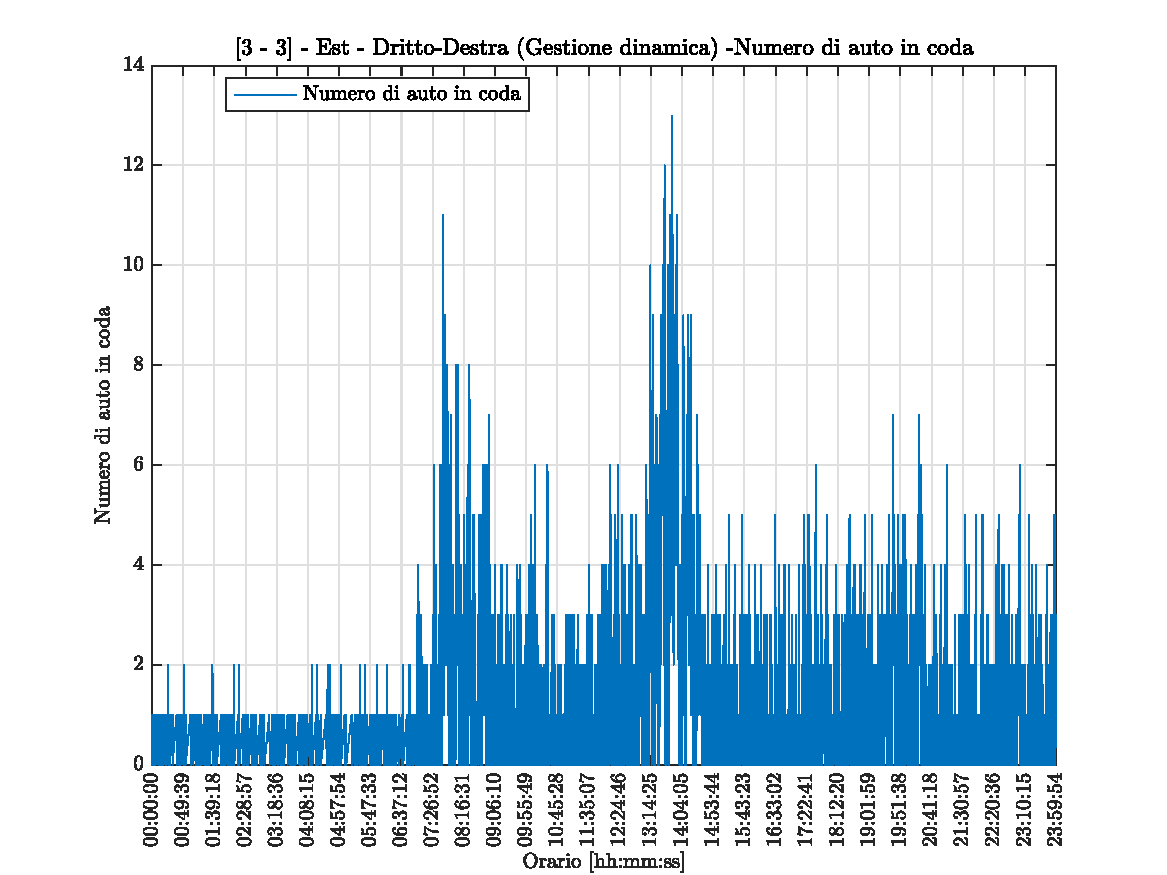
\includegraphics[width=0.9\textwidth]{cap4congestionemax.pdf}
  \caption{Variazione nel tempo del numero di auto in coda, corsia più congestionata della simulazione se gestita staticamente}
  \label{fig:}
\end{figure}
\begin{figure}[H]
\centering
  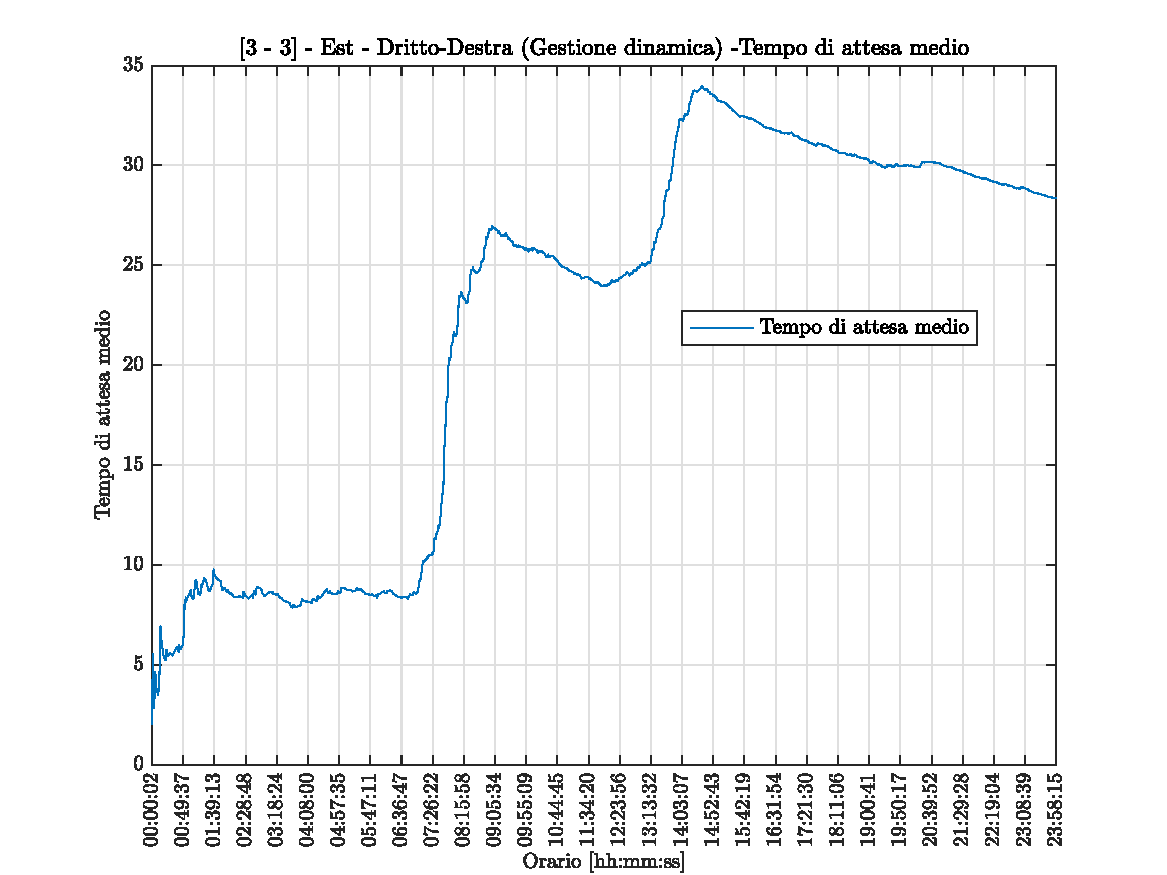
\includegraphics[width=0.9\textwidth]{cap4congestionetempi.pdf}
  \caption{Tempi di attesa in funzione della fascia oraria, corsia più congestionata della simulazione se gestita staticamente}
  \label{fig:}
\end{figure}
\begin{figure}[H]
\centering
  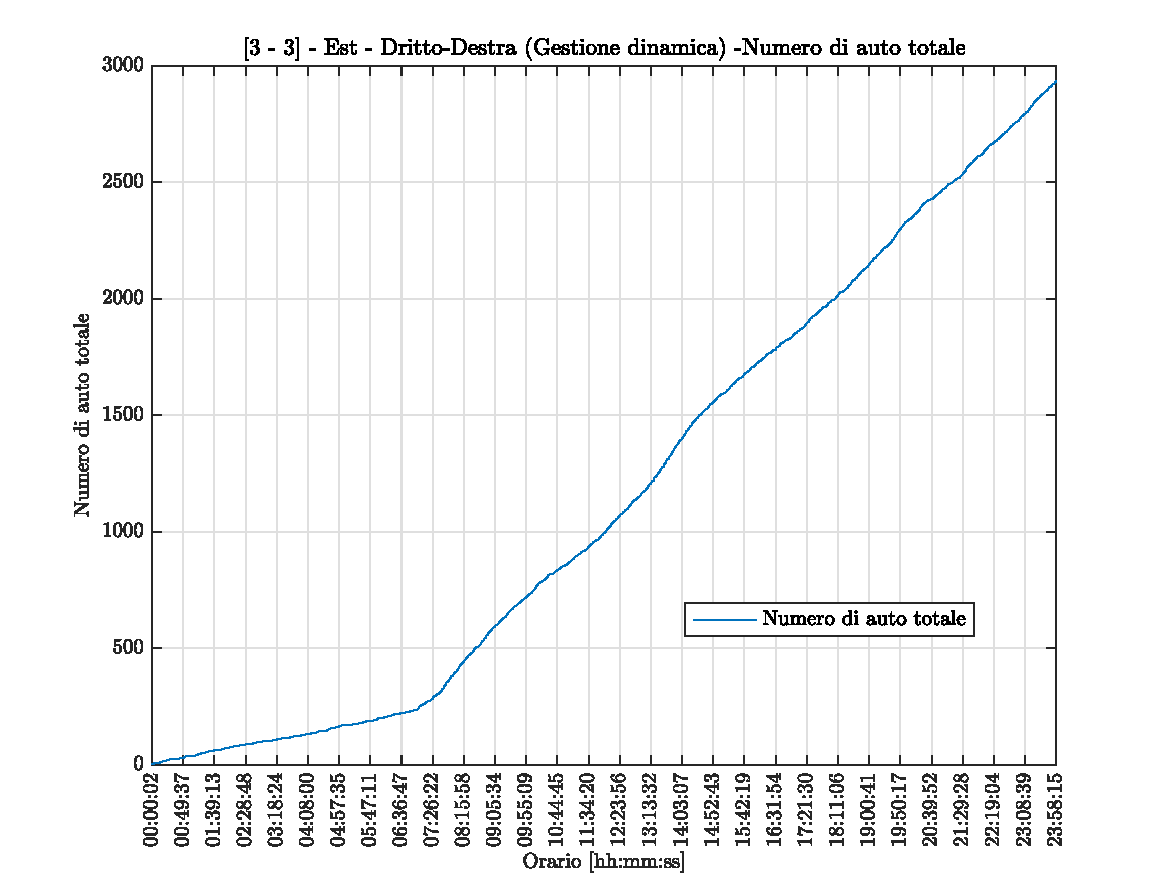
\includegraphics[width=0.9\textwidth]{cap4congestionenumauto.pdf}
  \caption{Numero complessivo di auto, corsia più congestionata della simulazione se gestita staticamente}
  \label{fig:}
\end{figure}
\newpage
Possiamo infatti notare che il massimo numero di auto in coda passa da 47 a 13, calando drasticamente a parità di tutte le altre condizioni. Anche il tempo medio di attesa si riduce notevolmente, da \textit{104.77s} a \textit{26.29s}. 

Un'obiezione di un lettore di questa tesi potrebbe riguardare il fatto che, per snellire questa corsia in particolare, altre subiscano un congestionamento. È bene dunque precisare che, complice l'introduzione del meccanismo di gestione della starvation presentato nei capitoli precedenti, nessuna strada viene trascurata. Dalla tabella, riassuntiva di quanto detto in questo capitolo si può notare, infatti, che ogni corsia, non importa di quale incrocio faccia parte o quale sia la sua tipoligia, viene amministrata in maniera ottimale, con risultati sempre migliori rispetto ad una gestione statica.
\newline
















